\section{Results}\label{sec:results}
% Outline row: results.tex. Table 2, Figures 4 and 5, the control night, the held-out result,
% the heart-rate adviser. Description only; interpretation is in the Discussion.

\begin{table}[t]\centering\footnotesize
\caption{Each induced low-oxygen recording replayed through the ship's rules. Warning: the last trend warning before the SOS. SOS: the first second with \numSustainN{} clean readings in a row at or below \numSpoTwoEmergency\%. Lead: SOS minus warning. Predicted left: the time left the ship stated at the warning. All times in seconds from the start of the recording.}\label{tab:events}
\setlength{\tabcolsep}{4pt}
% Written by scripts/paper_numbers.py. Do not edit by hand.
\begin{tabular}{@{}lrrrr@{}}\toprule
Recording & Warning (s) & SOS (s) & Lead (s) & Predicted left (s)\\ \midrule
100001 & 162 & 321 & 159 & 142 \\
100002 & 235 & 341 & 106 & 56 \\
100003 & 138 & 236 & 98 & 87 \\
100004 & 221 & 317 & 96 & 58 \\
100005 & 112 & 180 & 68 & 84 \\
100006 & 114 & 128 & 14 & 26 \\
\bottomrule\end{tabular}

\end{table}

\paragraph{Low-oxygen recordings.}
Table~\ref{tab:events} lists every event. In all \numUwEvents{} recordings the SpO$_2$ reached the emergency band, and in \numUwWarned{} of the \numUwEvents{} the ship raised a trend warning before the SOS. The lead ranged from \numUwMinLeadS{} to \numUwMaxLeadS~s, with a median of \numUwMedianLeadS~s (Figure~\ref{fig:evidence}, left). The counted warning came while the reading was still in the normal band in \numUwWarnNormalBandN{} of the \numUwEvents{} recordings (Figure~\ref{fig:event}). In the other recordings a caution or warning band was already held, so the fixed bands had already raised an alert and the warning added the time left to it. A trend warning came before the band rule's first caution in \numUwTrendBeforeCautionN{} of the \numUwEvents.

\begin{figure}[t]\centering
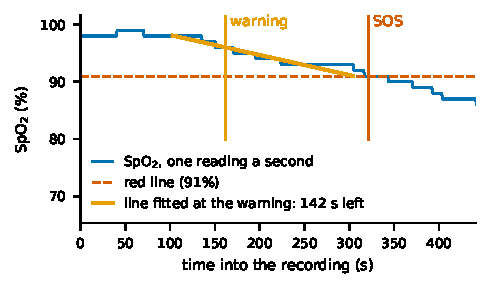
\includegraphics[width=\columnwidth]{figures/timeleft_event.pdf}
\caption{Recording 100001 of the induced low-oxygen data~\cite{hoffman2022oximetry}. The ship warned at the orange line and fitted the orange slope through the readings before it; the SOS (vermilion line) followed when \numSustainN{} readings in a row sat at or below the red line.}
\label{fig:event}
\end{figure}

The time left that the ship stated differed from the lead it actually had by a median of \numUwPredAbsErrMedianS~s and at most \numUwPredAbsErrMaxS~s. The stated time was shorter than the lead in \numUwPredShortN{} recordings and longer in \numUwPredLongN, by at most \numUwPredLongMaxS~s.

\paragraph{Held-out choice of settings.}
Of the \numGridSize{} settings in the grid, \numGridAllowed{} raised at most \numGridMaxControlWarnings{} trend warnings on the control night. In \numHeldoutRoundsShipSetting{} of the \numHeldoutRounds{} leave-one-out rounds, the setting chosen without the held-out recording was the one the ship runs (Table~\ref{tab:params}). Applied to the held-out recordings, the chosen settings warned before the SOS in \numHeldoutWarned{} of \numUwEvents, with a median lead of \numHeldoutMedianLeadS~s, the same as Table~\ref{tab:events}.

\begin{figure}[t]\centering
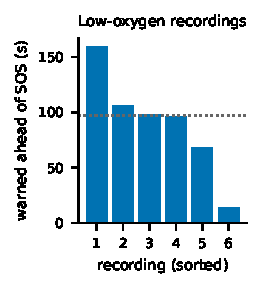
\includegraphics[width=0.49\columnwidth]{figures/lead_times.pdf}\hfill
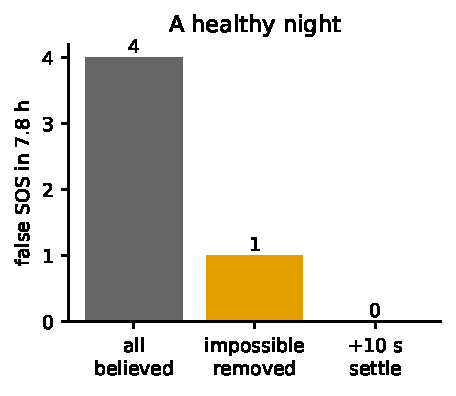
\includegraphics[width=0.49\columnwidth]{figures/false_sos.pdf}
\caption{Left: warning lead before the SOS in each of the \numUwEvents{} low-oxygen recordings, sorted; the dotted line is the median, \numUwMedianLeadS~s. Right: false SOS alarms on a healthy \numControlHours-hour night (Apnea-ECG \texttt{c01r}) with no trust rule, with the plausible-range check, and with the \numSettleN-reading settle count added.}
\label{fig:evidence}
\end{figure}

\paragraph{The healthy night.}
The control record held \numControlHours~hours of plausible SpO$_2$ readings. With every number believed, the band rule raised \numControlFalseSosRaw{} false SOS. Removing impossible numbers left \numControlFalseSosReject, and adding the settle count left \numControlFalseSosSettle{} (Figure~\ref{fig:evidence}, right). With the trend rule switched on, the same night raised \numControlTrendWarnings{} trend warnings. Each was a caution, the lowest level, and sent no SOS, but nothing was wrong with the sleeper, so we count both as false warnings.

\paragraph{The apnoea night.}
On the sleep-apnoea record (\numApneaHours~hours of plausible readings), the band rule raised an SOS \numApneaSosN{} times. A trend warning came within the \numApneaLookbackS~s before the SOS in \numApneaWarnedFirstN{} of them (\numApneaWarnedFirstPct\%), with a median lead of \numApneaMedianLeadS~s. In the rest, the SOS came from the fixed band alone.

\paragraph{The heart-rate adviser.}
Fitted on all \numHrPeople{} people, the adviser's limit was \numHrLimitBpm~beats a minute from the expected rate. Across the \numHrPeople{} leave-one-person-out rounds, the worst held-out person had \numHrWorstFlaggedMinPerH{} flagged minutes an hour, inside the gate of \numHrGateMinPerH. No recording contains an emergency, so this measures only how often it flags healthy people. The adviser is not wired into the ship.
